%% GENERATED by tools/from_docs.py from stepss-docs. Do not edit by hand:
%% edit the page named below in stepss-docs and regenerate.
%% source: stepss-docs/src/content/docs/models/exciters/generic.mdx

\chapter{Generic exciters}\label{doc:model-exc-generic}

Generic voltage regulators with optional stabilizer and limiter stages, and the regulator of a diesel generator. \texttt{GENERIC1} and \texttt{GENERIC2} are built in and written in uppercase with no prefix; \texttt{GENERIC} and \texttt{AVR\_DG} are registered, and RAMSES adds the \texttt{exc\_} prefix automatically.

The \texttt{EXC} sub-record these models are entered with, and the table of IEEE model variants, are on the \hyperref[doc:model-exc]{Exciter Models} page.

\section{\texorpdfstring{GENERIC1 (\texttt{exc\_generic1})}{GENERIC1 (exc\_generic1)}}\label{model-exc-generic:generic1-exc_generic1}

The data-file model name is \texttt{GENERIC1}.

\begin{figure}[htbp]
\centering
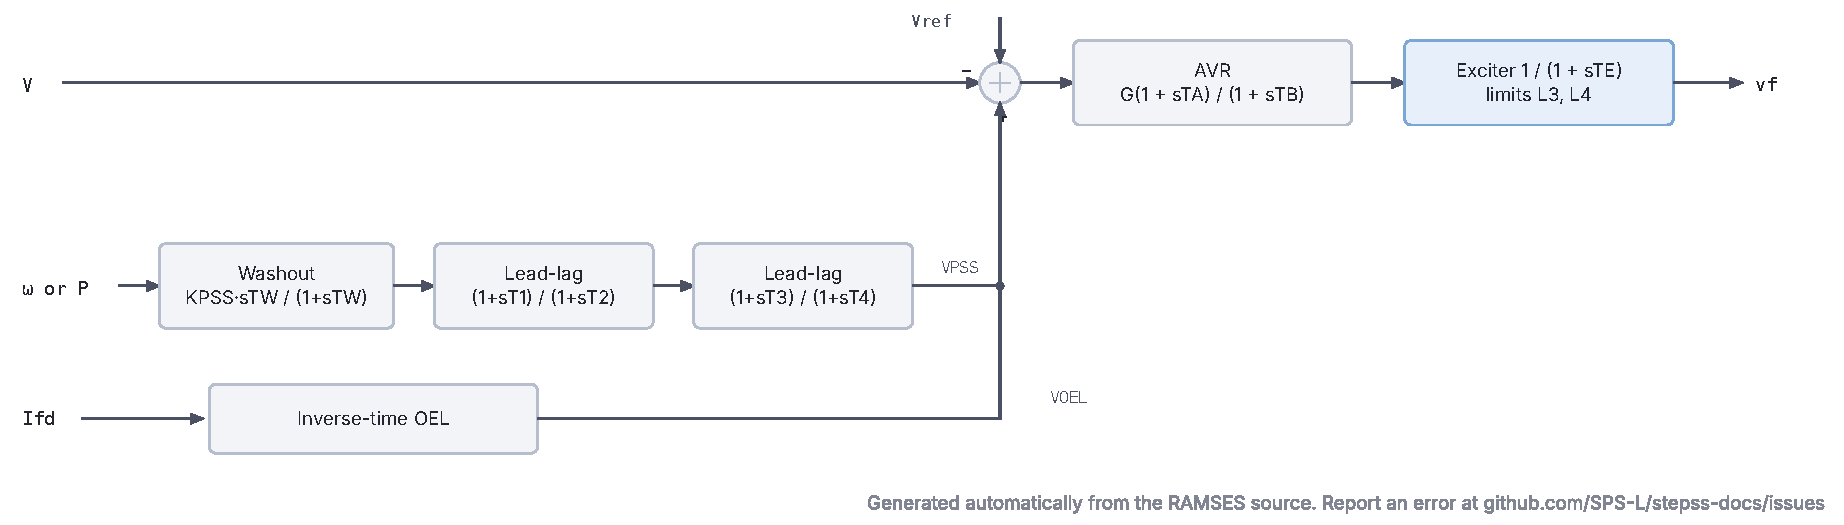
\includegraphics[width=0.98\linewidth]{figures/exc-generic1-light}
\caption{exc\_generic1 block diagram.}
\end{figure}

\subsection{Scientific Description}\label{model-exc-generic:scientific-description}

The \texttt{exc\_generic1} model is a \textbf{generic AVR with OEL (Over-Excitation Limiter) and PSS}, implemented in Fortran. It includes a proportional--integral AVR, a PSS acting on rotor speed or active power, and an inverse-time OEL.

\textbf{AVR:}

The excitation system uses a first-order integrating controller (washout or PI-type, set by the gain \(G\) and time constants \(T_A\), \(T_B\)) with output limits \([L_3,\, L_4]\):

\[V_f(s) = G \cdot \frac{1 + s T_A}{1 + s T_B} \cdot \left(V_{ref} - V\right) \cdot \frac{1}{1 + s T_E}\]

\textbf{PSS (speed or power input, selectable):}

Input signal is selected by \texttt{SPEEDIN}: 1 = rotor speed \(\omega\), 0 = electrical power \(P\).

\[V_{PSS}(s) = K_{PSS} \cdot \frac{s T_W}{1 + s T_W} \cdot \frac{1 + s T_1}{1 + s T_2} \cdot \frac{1 + s T_3}{1 + s T_4} \cdot u(s)\]

Output is clamped to \([DV_{MIN},\, DV_{MAX}]\).

\textbf{OEL (inverse-time limiter):}

The OEL monitors field current \(I_f\). When \(I_f > IFLIM\), a timer begins accumulating via:

\begin{itemize}
\tightlist
\item
  Dead zone \(d\) and phase \(f\) parameters control OEL activation thresholds.
\item
  The OEL integrates the overcurrent error and reduces \(V_{ref}\) once the timer reaches threshold \(L_1\), with output range \([L_1, L_2]\).
\end{itemize}

\textbf{Parameters from Fortran source} (\texttt{prm} array):

\begin{small}\begin{longtable}[]{@{}lll@{}}
\toprule\noalign{}
Index & Name & Description \\
\midrule\noalign{}
\endhead
\bottomrule\noalign{}
\endlastfoot
1 & \texttt{IFLIM} & Field current OEL threshold (pu) \\
2 & \texttt{d} & OEL dead zone (pu) \\
3 & \texttt{f} & OEL phase characteristic \\
4 & \texttt{S} & AVR setpoint input (usually 0 = \(V\)) \\
5 & \texttt{K1} & AVR lead numerator gain \\
6 & \texttt{K2} & AVR lag denominator gain \\
7 & \texttt{L1} & OEL integrator lower limit (pu) \\
8 & \texttt{L2} & OEL integrator upper limit (pu) \\
9 & \texttt{G} & AVR overall gain \\
10 & \texttt{TA} & AVR lead time constant (s) \\
11 & \texttt{TB} & AVR lag time constant (s) \\
12 & \texttt{TE} & Exciter time constant (s) \\
13 & \texttt{L3} & AVR output lower limit (pu) \\
14 & \texttt{L4} & AVR output upper limit (pu) \\
15 & \texttt{SPEEDIN} & PSS input signal: 1 = speed, 0 = power \\
16 & \texttt{KPSS} & PSS gain \\
17 & \texttt{Tw} & PSS washout time constant (s) \\
18 & \texttt{T1} & PSS lead--lag 1 zero (s) \\
19 & \texttt{T2} & PSS lead--lag 1 pole (s) \\
20 & \texttt{T3} & PSS lead--lag 2 zero (s) \\
21 & \texttt{T4} & PSS lead--lag 2 pole (s) \\
22 & \texttt{DVMIN} & PSS output lower limit (pu) \\
23 & \texttt{DVMAX} & PSS output upper limit (pu) \\
\end{longtable}\end{small}

\subsection{Usage Example}\label{model-exc-generic:usage-example}

\textbf{RAMSES Data File}

\begin{Verbatim}
SYNC_MACH  GEN1  BUS1
      # FP FQ P Q: share of the power-flow injection (FP, FQ) or initial power (P in MW, Q in Mvar)
      1.  1.  0.  0.
      # SNOM: Nominal apparent power, used as base power in the machine model (MVA)
      600.
      # Pnom: Nominal active power of the turbine, used as base power for the turbine model (MW)
      570.
      # H: Inertia constant (s)
      3.
      # D: Damping coefficient (usually set to zero when the damper windings are modelled) (pu)
      0.
      # IBRATIO: Field current base ratio I_fB^mac/I_fB^exc (see above) (pu)
      0.95
      # TYPE_MOD: Parameter format keyword: RL or XT (case-insensitive)
      XT
      # Xl: Leakage reactance L_l (pu)
      0.15
      # Xd: d-axis synchronous reactance (pu)
      1.1
      # X'd: d-axis transient reactance (must be smaller than Xd) (pu)
      0.25
      # X"d: d-axis subtransient reactance (pu)
      0.2
      # Xq: q-axis synchronous reactance (pu)
      0.7
      # X'q: q-axis transient reactance (pu)
      *
      # X"q: q-axis subtransient reactance (pu)
      0.2
      # m: Saturation coefficient (set to 0 to neglect saturation)
      0.1
      # n: Saturation exponent (ignored when m = 0)
      6.0257
      # Ra: Armature resistance (pu)
      0.
      # T'do: d-axis open-circuit transient time constant (s)
      5.00
      # T"do: d-axis open-circuit subtransient time constant (s)
      0.05
      # T'qo: q-axis open-circuit transient time constant (s)
      *
      # T"qo: q-axis open-circuit subtransient time constant (s)
      0.1
EXC  GENERIC1
      # IFLIM: OEL field current threshold (pu)
      1.05
      # d: OEL timer band, usually negative: timer runs down at rate 1 below IFLIM+d, holds between IFLIM+d and IFLIM (pu)
      -0.1
      # f: OEL timer charging rate offset above IFLIM
      0.5
      # S: OEL timer charging rate per unit of field overcurrent (1/pu)
      0.0
      # K1: Not used by the code
      1.0
      # K2: OEL gain on (if - IFLIM), negative so that the OEL lowers excitation (pu/pu)
      -1.0
      # L1: OEL timer lower limit and initial value, negative; the OEL acts when the timer exceeds 0 (s)
      -20.
      # L2: OEL timer upper limit (s)
      0.5
      # G: AVR gain (pu/pu)
      200.0
      # TA: AVR lead time constant (s)
      0.02
      # TB: AVR lag time constant (s)
      0.10
      # TE: Exciter time constant (s)
      0.05
      # L3: Minimum field voltage (pu)
      0.0
      # L4: Maximum field voltage (pu)
      6.0
      # SPEEDIN: PSS input weight: 1 = speed, 0 = active power
      1
      # KPSS: PSS gain, derivative washout KPSS s/(1+sTw); 0 disables PSS (pu s)
      9.5
      # Tw: PSS washout time constant (s)
      1.40
      # T1: PSS first lead-lag numerator time constant (s)
      0.15
      # T2: PSS first lead-lag denominator time constant (s)
      0.03
      # T3: PSS second lead-lag numerator time constant (s)
      0.15
      # T4: PSS second lead-lag denominator time constant (s)
      0.03
      # DVMIN: PSS output lower limit (pu)
      -0.10
      # DVMAX: PSS output upper limit (pu)
      0.10
TOR  CONSTANT
;
\end{Verbatim}

\begin{center}\rule{0.5\linewidth}{0.5pt}\end{center}

\section{\texorpdfstring{AVR\_DG (\texttt{exc\_AVR\_DG})}{AVR\_DG (exc\_AVR\_DG)}}\label{model-exc-generic:avr_dg-exc_avr_dg}

The data-file model name is \texttt{AVR\_DG}. Registered since 3.76.

\begin{figure}[htbp]
\centering
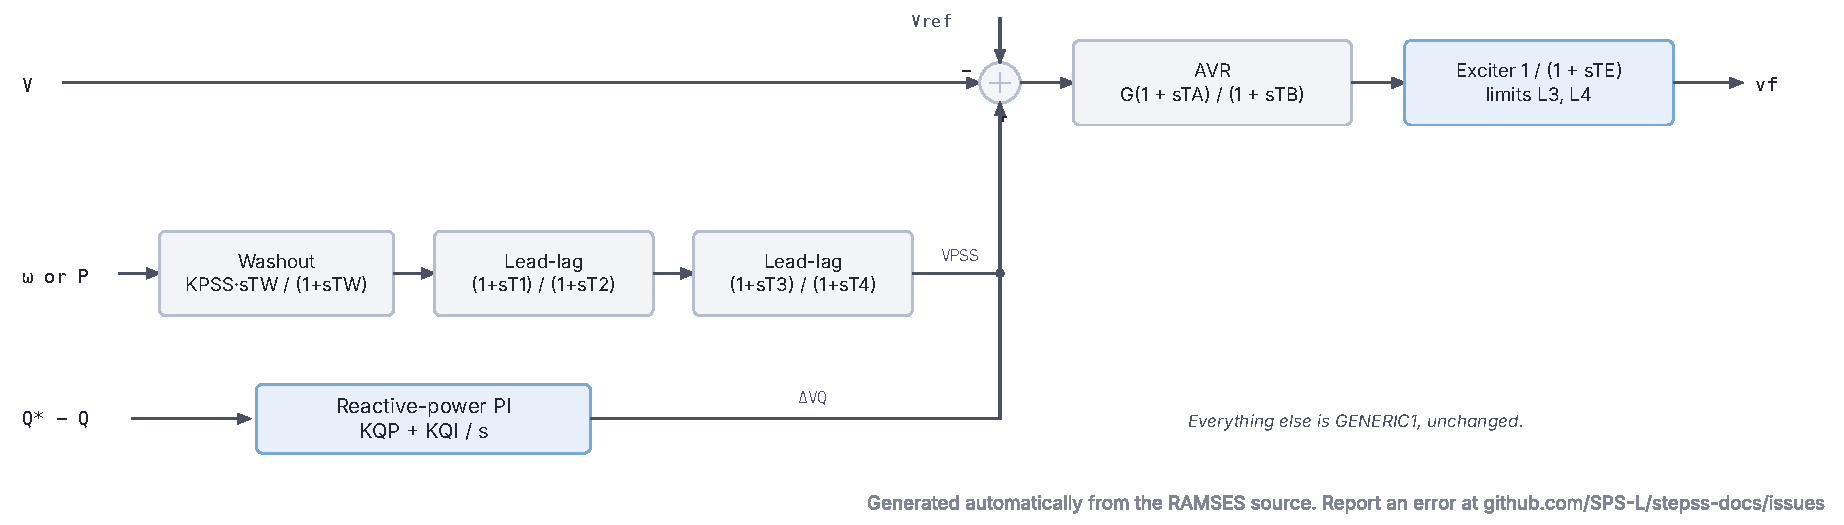
\includegraphics[width=0.98\linewidth]{figures/exc-avr-dg-light}
\caption{exc\_AVR\_DG block diagram.}
\end{figure}

\subsection{Scientific Description}\label{model-exc-generic:scientific-description-1}

An AVR for \textbf{dispersed generation}: the \hyperref[model-exc-generic:generic1-exc_generic1]{\texttt{GENERIC1}} excitation
system, OEL and PSS, plus a \textbf{reactive-power PI controller} that trims the voltage
reference so the unit holds a reactive-power setpoint.

Parameters 1 to 23 are those of \texttt{GENERIC1}, in the same positions and with the same
meanings, and the AVR, PSS and OEL behave identically. Only the summing junction changes,
gaining a third contribution:

\[e = V_{ref} - V + \Delta V_{PSS} + \Delta V_{Q}\]

\textbf{Reactive-power regulator:}

The error is the deviation from the setpoint captured at initialisation:

\[\dot{x}_{Q} = K_{QI} \left(Q^{*} - Q\right), \qquad
\Delta V_{Q} = K_{QP} \left(Q^{*} - Q\right) + x_{Q}\]

clamped to \([L_5,\, L_6]\). Setting \(K_{QP} = K_{QI} = 0\) leaves the loop dormant and the
model reduces to \texttt{GENERIC1}.

\textbf{Parameters:}

Indices 1 to 23 are exactly those of \hyperref[model-exc-generic:generic1-exc_generic1]{\texttt{GENERIC1}}. The four that
follow are new:

\begin{small}\begin{longtable}[]{@{}lll@{}}
\toprule\noalign{}
Index & Name & Description \\
\midrule\noalign{}
\endhead
\bottomrule\noalign{}
\endlastfoot
24 & \texttt{KQP} & Reactive-power regulator proportional gain \\
25 & \texttt{KQI} & Reactive-power regulator integral gain \\
26 & \texttt{L5} & Regulator output lower limit (pu) \\
27 & \texttt{L6} & Regulator output upper limit (pu) \\
\end{longtable}\end{small}

\textbf{Implementation details:}
- \texttt{nbxvar\ =\ 8}, \texttt{nbzvar\ =\ 7}, \texttt{nbdata\ =\ 27}, \texttt{nbaddpar\ =\ 2}
- Additional: \texttt{prm(28)\ =\ V0} (voltage reference) and \texttt{prm(29)\ =\ Qset}, both captured at
initialisation
- Observables: those of \texttt{GENERIC1} plus \texttt{deltavq} and \texttt{Qset}

\subsection{Usage Example}\label{model-exc-generic:usage-example-1}

\textbf{RAMSES Data File}

\begin{Verbatim}
SYNC_MACH  G4  N4
      # FP FQ P Q: share of the power-flow injection (FP, FQ) or initial power (P in MW, Q in Mvar)
      1.  1.  0.  0.
      # SNOM: Nominal apparent power, used as base power in the machine model (MVA)
      5
      # Pnom: Nominal active power of the turbine, used as base power for the turbine model (MW)
      4.5
      # H: Inertia constant (s)
      3.
      # D: Damping coefficient (usually set to zero when the damper windings are modelled) (pu)
      0.
      # IBRATIO: Field current base ratio I_fB^mac/I_fB^exc (see above) (pu)
      1.9333
      # TYPE_MOD: Parameter format keyword: RL or XT (case-insensitive)
      XT
      # Xl: Leakage reactance L_l (pu)
      0.0937
      # Xd: d-axis synchronous reactance (pu)
      2.027
      # X'd: d-axis transient reactance (must be smaller than Xd) (pu)
      0.210
      # X"d: d-axis subtransient reactance (pu)
      0.173
      # Xq: q-axis synchronous reactance (pu)
      2.027
      # X'q: q-axis transient reactance (pu)
      *
      # X"q: q-axis subtransient reactance (pu)
      0.173
      # m: Saturation coefficient (set to 0 to neglect saturation)
      0.1
      # n: Saturation exponent (ignored when m = 0)
      6
      # Ra: Armature resistance (pu)
      0.00
      # T'do: d-axis open-circuit transient time constant (s)
      3.1
      # T"do: d-axis open-circuit subtransient time constant (s)
      0.0387
      # T'qo: q-axis open-circuit transient time constant (s)
      *
      # T"qo: q-axis open-circuit subtransient time constant (s)
      0.0387
EXC  AVR_DG
      # IFLIM: OEL field current threshold (pu)
      2.865
      # d: OEL timer band, usually negative: timer runs down at rate 1 below IFLIM+d, holds between IFLIM+d and IFLIM (pu)
      -0.1
      # f: OEL timer charging rate offset above IFLIM
      0.
      # S: OEL timer charging rate per unit of field overcurrent (1/pu)
      1.
      # K1: Not used by the code
      100.
      # K2: OEL gain on field current error if minus IFLIM (pu/pu)
      -1.
      # L1: OEL timer lower limit (initial value) (s)
      -20
      # L2: OEL timer upper limit (s)
      10
      # G: AVR gain (pu/pu)
      50
      # TA: AVR lead time constant (s)
      4
      # TB: AVR lag time constant (s)
      20
      # TE: Exciter time constant (s)
      0.1
      # L3: Minimum field voltage (pu)
      0
      # L4: Maximum field voltage (pu)
      5
      # SPEEDIN: PSS input weight: 1 = speed, 0 = active power
      1
      # KPSS: PSS gain, derivative washout KPSS s/(1+sTw); 0 disables PSS (pu s)
      0.
      # Tw: PSS washout time constant (s)
      5.
      # T1: PSS first lead-lag numerator time constant (s)
      1.
      # T2: PSS first lead-lag denominator time constant (s)
      1.
      # T3: PSS second lead-lag numerator time constant (s)
      1.
      # T4: PSS second lead-lag denominator time constant (s)
      1.
      # DVMIN: PSS output lower limit (pu)
      0.
      # DVMAX: PSS output upper limit (pu)
      0.
      # KQP: Reactive power regulator proportional gain (pu/pu)
      0.04
      # KQI: Reactive power regulator integral gain (1/s)
      0.06
      # L5: Reactive power regulator output lower limit (pu)
      -0.2
      # L6: Reactive power regulator output upper limit (pu)
      0.33
TOR  HYDRO_DG
      # Qv: no-load water flow (pu)
      0.0
      # Kp: PI proportional gain on power error
      0.1
      # Ki: PI integral gain on power error (1/s)
      0.4
      # TSM: gate servomotor time constant (s)
      0.2
      # LIMZDOT: gate velocity limit, applied as plus or minus (pu/s)
      0.1
      # TW: water starting time (s)
      1.0
;
\end{Verbatim}

\textbf{Notes}

\begin{itemize}
\tightlist
\item
  The setpoint is \textbf{not} a parameter. \texttt{Qset} is captured from the power-flow solution at
  initialisation, so the unit holds whatever reactive power it was dispatched at.
\item
  With \texttt{KQP} and \texttt{KQI} non-zero the unit regulates reactive power rather than terminal
  voltage, which is the usual arrangement for dispersed generation connected to a
  distribution network under a connection agreement.
\item
  \texttt{KPSS\ =\ 0} disables the stabiliser. Note that this drives the PSS branch to its lower
  limit, so \texttt{DVMIN} should be 0 as well, as in the example above.
\item
  Pair it with \hyperref[doc:model-tor-generic]{\texttt{HYDRO\_DG}} for a unit that
  regulates both its active and reactive power and provides no primary frequency response.
\end{itemize}

\begin{center}\rule{0.5\linewidth}{0.5pt}\end{center}

\section{\texorpdfstring{GENERIC2 (\texttt{exc\_generic2})}{GENERIC2 (exc\_generic2)}}\label{model-exc-generic:generic2-exc_generic2}

The data-file model name is \texttt{GENERIC2}.

\begin{figure}[htbp]
\centering
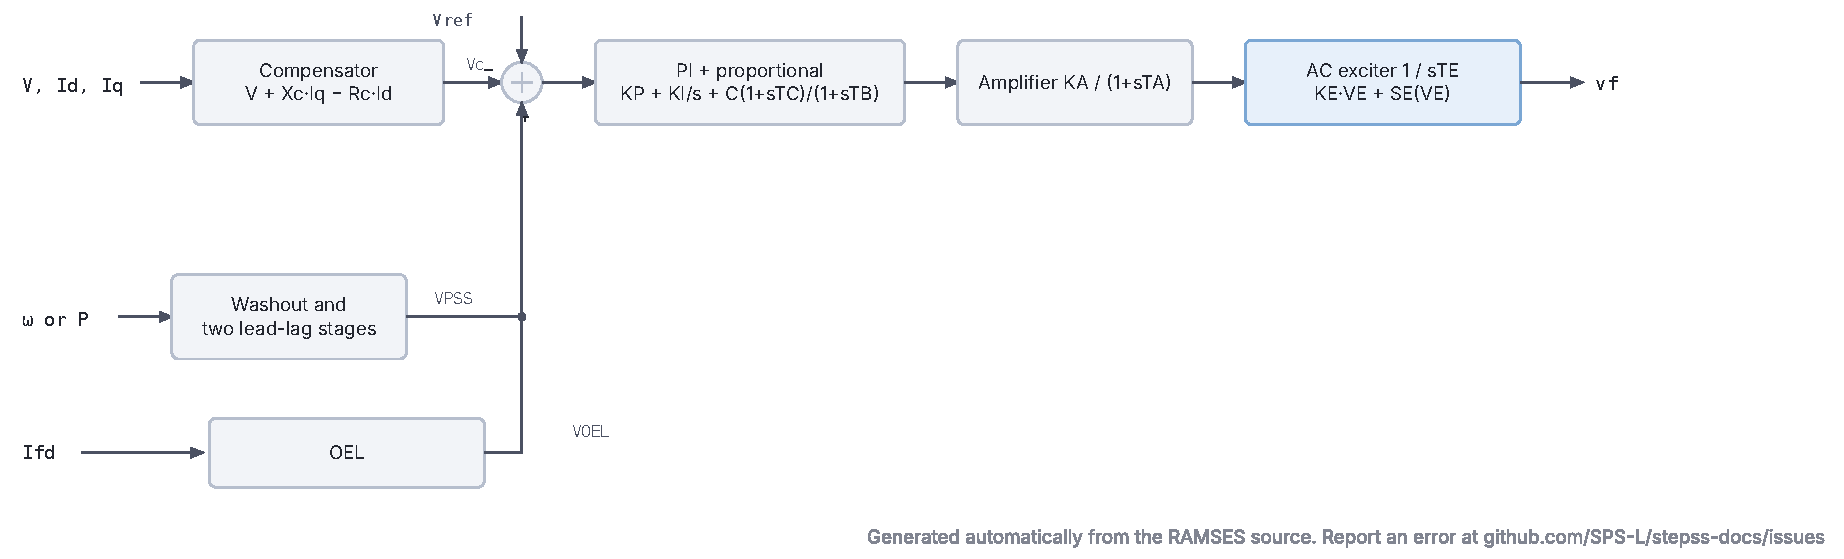
\includegraphics[width=0.98\linewidth]{figures/exc-generic2-light}
\caption{exc\_generic2 block diagram.}
\end{figure}

\subsection{Scientific Description}\label{model-exc-generic:scientific-description-2}

The \texttt{exc\_generic2} model is a more detailed \textbf{generic AVR}. It includes a voltage compensator, a combined PI--proportional regulator, an AC exciter with saturation, a PSS, and an OEL.

\textbf{Voltage measurement with line-drop compensation:}

\[V_c = V + X_c \cdot I_q - R_c \cdot I_d \quad (\text{or simplified})\]

\textbf{PI--proportional AVR with transient gain reduction:}

\[V_{AVR}(s) = \left(K_P + \frac{K_I}{s} + C \cdot \frac{1 + s T_C}{1 + s T_B}\right) \cdot K_A \cdot \frac{1}{1 + s T_A}(V_{ref} - V_c)\]

\textbf{AC exciter with saturation:}

\[\frac{d V_E}{dt} = \frac{1}{T_E}\left[V_R - K_E \cdot V_E - S_E(V_E)\right]\]

where \(S_E(V_E)\) is the piecewise-linear saturation function defined by \((E_1, S_{E1})\) and \((E_2, S_{E2})\).

\textbf{PSS (type selectable by \texttt{typss}):}

\[V_s(s) = K_{PSS} \cdot \frac{s T_W}{1 + s T_W} \cdot \frac{1 + s T_1}{1 + s T_2} \cdot \frac{1 + s T_3}{1 + s T_4} \cdot u(s)\]

\textbf{OEL (inverse-time, three-segment):}

The OEL uses a three-level piecewise-linear characteristic \((s_1, T_{oel1})\), \((s_2, T_{oel2})\), \((s_3, T_{oel3})\) to compute the allowable overcurrent time.

\textbf{Parameters from Fortran \texttt{associate} block} (39 data parameters + 4 additional):

\begin{small}\begin{longtable}[]{@{}lll@{}}
\toprule\noalign{}
Index & Name & Description \\
\midrule\noalign{}
\endhead
\bottomrule\noalign{}
\endlastfoot
1 & \texttt{Xc} & Line-drop compensation reactance (pu) \\
2 & \texttt{Tr} & Voltage measurement time constant (s) \\
3 & \texttt{C} & TGR numerator gain \\
4 & \texttt{Tc} & TGR lead time constant (s) \\
5 & \texttt{Tb} & TGR lag time constant (s) \\
6 & \texttt{Ka} & AVR proportional gain \\
7 & \texttt{Ta} & AVR time constant (s) \\
8 & \texttt{Ki} & AVR integral gain \\
9 & \texttt{Kp} & AVR proportional path gain \\
10 & \texttt{VrmaxD} & Regulator max (dynamic, pu) \\
11 & \texttt{VrminD} & Regulator min (dynamic, pu) \\
12 & \texttt{G} & Exciter overall gain \\
13 & \texttt{Ke} & Exciter self-excitation coefficient \\
14 & \texttt{Te} & Exciter time constant (s) \\
15 & \texttt{E1} & Saturation breakpoint 1 (pu) \\
16 & \texttt{SeE1} & Saturation factor at \(E_1\) \\
17 & \texttt{E2} & Saturation breakpoint 2 (pu) \\
18 & \texttt{SeE2} & Saturation factor at \(E_2\) \\
19 & \texttt{Vrmax} & Field voltage upper limit (pu) \\
20 & \texttt{Vrmin} & Field voltage lower limit (pu) \\
21 & \texttt{typss} & PSS input type (1 = speed, 2 = power) \\
22 & \texttt{W} & PSS input gain \\
23 & \texttt{Tf} & PSS derivative filter time constant (s) \\
24 & \texttt{Kpss} & PSS gain \\
25 & \texttt{Tw} & PSS washout time constant (s) \\
26 & \texttt{T1} & PSS lead--lag 1 zero (s) \\
27 & \texttt{T2} & PSS lead--lag 1 pole (s) \\
28 & \texttt{T3} & PSS lead--lag 2 zero (s) \\
29 & \texttt{T4} & PSS lead--lag 2 pole (s) \\
30 & \texttt{Lim} & PSS output symmetric limit (pu) \\
31 & \texttt{LimSup} & PSS upper asymmetric limit (pu) \\
32 & \texttt{s1} & OEL segment 1 (pu \(I_f\)) \\
33 & \texttt{toel1} & OEL time at segment 1 (s) \\
34 & \texttt{s2} & OEL segment 2 (pu \(I_f\)) \\
35 & \texttt{toel2} & OEL time at segment 2 (s) \\
36 & \texttt{s3} & OEL segment 3 (pu \(I_f\)) \\
37 & \texttt{toel3} & OEL time at segment 3 (s) \\
38 & \texttt{perm} & OEL permanent current limit (pu) \\
39 & \texttt{LimInf} & PSS lower asymmetric limit (pu) \\
\end{longtable}\end{small}

\subsection{Usage Example}\label{model-exc-generic:usage-example-2}

\textbf{RAMSES Data File}

\begin{Verbatim}
SYNC_MACH  GEN1  BUS1
      # FP FQ P Q: share of the power-flow injection (FP, FQ) or initial power (P in MW, Q in Mvar)
      1.  1.  0.  0.
      # SNOM: Nominal apparent power, used as base power in the machine model (MVA)
      600.
      # Pnom: Nominal active power of the turbine, used as base power for the turbine model (MW)
      570.
      # H: Inertia constant (s)
      3.
      # D: Damping coefficient (usually set to zero when the damper windings are modelled) (pu)
      0.
      # IBRATIO: Field current base ratio I_fB^mac/I_fB^exc (see above) (pu)
      0.95
      # TYPE_MOD: Parameter format keyword: RL or XT (case-insensitive)
      XT
      # Xl: Leakage reactance L_l (pu)
      0.15
      # Xd: d-axis synchronous reactance (pu)
      1.1
      # X'd: d-axis transient reactance (must be smaller than Xd) (pu)
      0.25
      # X"d: d-axis subtransient reactance (pu)
      0.2
      # Xq: q-axis synchronous reactance (pu)
      0.7
      # X'q: q-axis transient reactance (pu)
      *
      # X"q: q-axis subtransient reactance (pu)
      0.2
      # m: Saturation coefficient (set to 0 to neglect saturation)
      0.1
      # n: Saturation exponent (ignored when m = 0)
      6.0257
      # Ra: Armature resistance (pu)
      0.
      # T'do: d-axis open-circuit transient time constant (s)
      5.00
      # T"do: d-axis open-circuit subtransient time constant (s)
      0.05
      # T'qo: q-axis open-circuit transient time constant (s)
      *
      # T"qo: q-axis open-circuit subtransient time constant (s)
      0.1
EXC  GENERIC2
      # Xc: Compensation reactance (pu)
      0.0
      # Tr: Voltage measurement time constant, 0 = algebraic (s)
      0.02
      # C: Forward path selector: 0 = PI (Ki, Kp), 1 = lead-lag (Tc, Tb)
      1.0
      # Tc: Lead-lag numerator time constant, used when C = 1 (s)
      0.10
      # Tb: Lead-lag denominator time constant, used when C = 1 (s)
      1.00
      # Ka: Amplifier gain (pu/pu)
      200.0
      # Ta: Amplifier time constant, 0 = algebraic (s)
      0.05
      # Ki: PI integral gain, used when C = 0 (1/s)
      5.0
      # Kp: PI proportional gain, used when C = 0 (pu/pu)
      1.0
      # VrmaxD: Amplifier output upper limit (pu)
      6.0
      # VrminD: Amplifier output lower limit (pu)
      -6.0
      # G: Exciter selector: 1 = static (vf from amplifier), 0 = rotating exciter
      1.0
      # Ke: Exciter self-excitation constant (pu)
      1.0
      # Te: Exciter time constant (s)
      0.50
      # E1: First saturation point field voltage (pu)
      3.10
      # SeE1: Saturation factor at E1
      0.066
      # E2: Second saturation point field voltage (pu)
      4.18
      # SeE2: Saturation factor at E2
      0.91
      # Vrmax: Field voltage upper limit, multiplied by terminal voltage (pu)
      6.0
      # Vrmin: Field voltage lower limit, multiplied by terminal voltage (pu)
      -6.0
      # typss: PSS input: 0 = none, 1 = speed deviation, 2 = active power, 3 = filtered speed derivative
      1.0
      # W: PSS washout switch: 1 = washout, otherwise pure gain
      1.0
      # Tf: Speed derivative filter time constant, used when typss = 3 (s)
      0.05
      # Kpss: PSS gain; with W = 1 the washout is Kpss s/(1+sTw) and Kpss must be nonzero
      9.5
      # Tw: PSS washout time constant (s)
      1.40
      # T1: PSS first lead-lag numerator time constant (s)
      0.154
      # T2: PSS first lead-lag denominator time constant (s)
      0.033
      # T3: PSS second lead-lag numerator time constant (s)
      0.154
      # T4: PSS second lead-lag denominator time constant (s)
      0.033
      # Lim: PSS output symmetric limit (pu)
      0.10
      # LimSup: OEL field current above which the OEL acts without delay; highest threshold (pu)
      2.0
      # s1: OEL upper threshold, below LimSup (pu)
      1.5
      # toel1: OEL delay for field current between s1 and LimSup (s)
      10.
      # s2: OEL middle threshold, below s1 (pu)
      1.2
      # toel2: OEL delay for field current between s2 and s1 (s)
      60.
      # s3: OEL pickup, the lowest threshold; the timer starts above it (pu)
      1.1
      # toel3: OEL delay for field current between s3 and s2 (s)
      200.
      # perm: Field voltage ceiling applied once the OEL has acted (pu)
      1.05
      # LimInf: Field current below which field voltage is floored at LimInf (pu)
      -0.10
TOR  CONSTANT
;
\end{Verbatim}

\begin{center}\rule{0.5\linewidth}{0.5pt}\end{center}

\section{\texorpdfstring{GENERIC (\texttt{exc\_GENERIC})}{GENERIC (exc\_GENERIC)}}\label{model-exc-generic:generic-exc_generic}

The data-file model name is \texttt{exc\_GENERIC} (or \texttt{GENERIC}. The \texttt{exc\_} prefix is added automatically).

\begin{docsnote}{Renamed in RAMSES 3.57}

This model was called \texttt{exc\_GENERIC3} up to and including 3.56, and a second
registered name, \texttt{exc\_GENERIC4}, resolved to a byte-for-byte copy of it. Both
names were removed in 3.57 in favour of the single name \texttt{exc\_GENERIC}.

On 3.57 and later, a record naming \texttt{exc\_GENERIC3} or \texttt{exc\_GENERIC4} stops with
\texttt{Excitation\ model\ not\ found\ in\ definition}. Change it to \texttt{exc\_GENERIC}; the 20
data parameters and their order are unchanged, so nothing else in the record
moves.

\end{docsnote}

\begin{figure}[htbp]
\centering
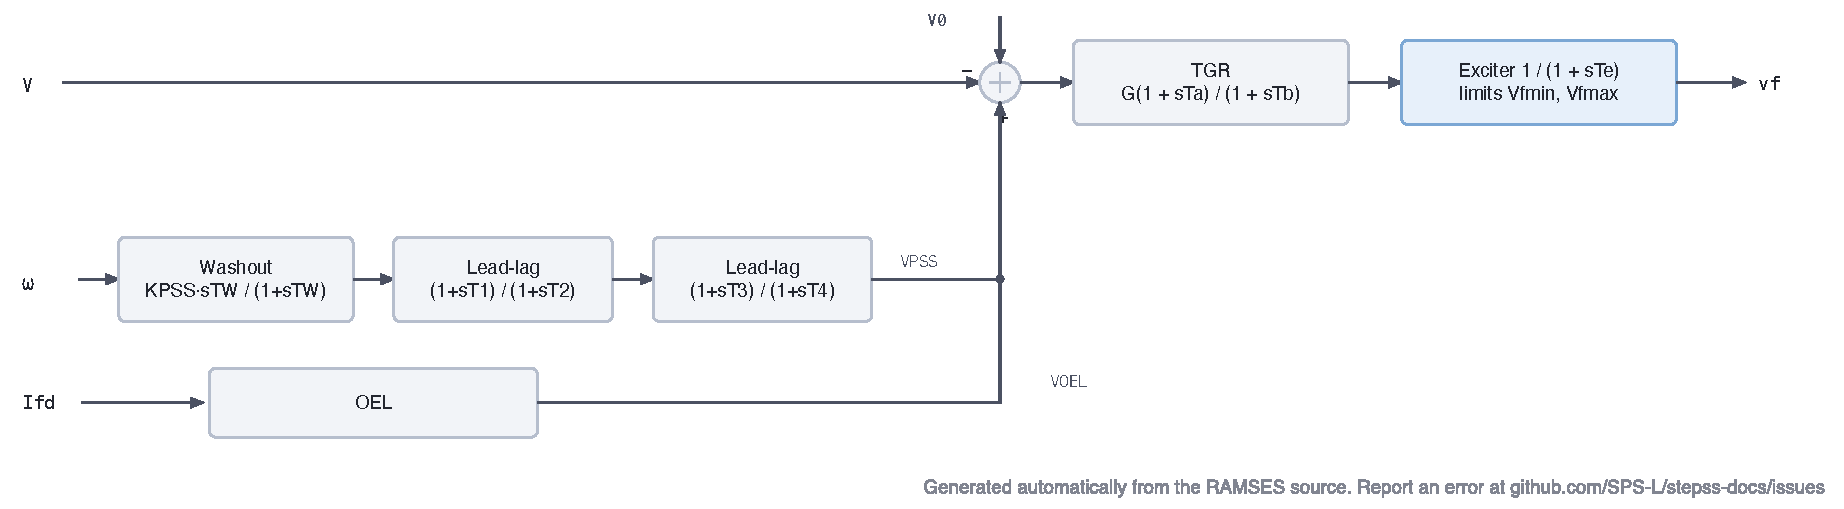
\includegraphics[width=0.98\linewidth]{figures/exc-generic-light}
\caption{exc\_GENERIC block diagram.}
\end{figure}

\subsection{Scientific Description}\label{model-exc-generic:scientific-description-3}

The \texttt{exc\_GENERIC} model (note capital letters) is a \textbf{generic AVR with integrated PSS and OEL}, defined via the CODEGEN \texttt{.txt} description. It provides a clean, modular three-block structure: AVR, PSS, and OEL.

\textbf{AVR (transient gain reduction + exciter):}

\[\Delta V = V_0 - V + V_{PSS} - V_{OEL}\]

\[V_1(s) = G \cdot \frac{1 + s T_a}{1 + s T_b} \cdot \Delta V(s)\]

\[V_f(s) = \frac{1}{1 + s T_e} \cdot V_1(s), \quad V_f \in [V_{f,min},\, V_{f,max}]\]

where \(V_0 = V + V_f/G\) is computed at initialisation.

\textbf{PSS (washout + two lead--lag stages):}

\[V_{PSS}(s) = \frac{K_{PSS} \cdot s T_W}{1 + s T_W} \cdot \frac{1 + s T_1}{1 + s T_2} \cdot \frac{1 + s T_3}{1 + s T_4} \cdot \omega(s)\]

Output is limited to \([-C,\, +C]\).

\textbf{OEL (inverse-time integrator):}

\[x_{oel1} = I_f - if_{1lim}\]

\[\frac{d x_{oel2}}{dt} = \frac{1}{T_{oel}} \cdot \min(x_{oel1},\, if_{2lim}), \quad x_{oel2} \in [L_1,\, L_2]\]

\[V_{OEL} = \text{clip}(K_{oel} \cdot x_{oel2},\, 0,\, L_3)\]

The CODEGEN block structure from the \texttt{.txt} file:

\begin{small}\begin{longtable}[]{@{}
  >{\raggedright\arraybackslash}p{(\linewidth - 6\tabcolsep) * \real{0.3529}}
  >{\raggedright\arraybackslash}p{(\linewidth - 6\tabcolsep) * \real{0.2321}}
  >{\raggedright\arraybackslash}p{(\linewidth - 6\tabcolsep) * \real{0.4149}}
@{}}
\toprule\noalign{}
\begin{minipage}[b]{\linewidth}\raggedright
Block
\end{minipage} & \begin{minipage}[b]{\linewidth}\raggedright
CODEGEN type
\end{minipage} & \begin{minipage}[b]{\linewidth}\raggedright
Signal
\end{minipage} \\
\midrule\noalign{}
\endhead
\bottomrule\noalign{}
\endlastfoot
AVR summing junction & \texttt{algeq} & \(V_0 - V + dv_{PSS} - dv_{OEL} - \Delta V\) \\
Transient gain reduction & \texttt{tf1p1z} & \(G(1+sT_a)/(1+sT_b)\) \\
Exciter & \texttt{tf1plim} & \(1/(1+sT_e)\) with \([V_{f,min}, V_{f,max}]\) \\
PSS washout & \texttt{tfder1p} & \(K_{PSS} \cdot sT_W / (1+sT_W)\) \\
PSS lead--lag 1 & \texttt{tf1p1z} & \((1+sT_1)/(1+sT_2)\) \\
PSS lead--lag 2 & \texttt{tf1p1z} & \((1+sT_3)/(1+sT_4)\) \\
PSS limiter & \texttt{lim} & \([-C, +C]\) \\
OEL error & \texttt{algeq} & \(I_f - if_{1lim}\) \\
OEL upper bound & \texttt{min1v1c} & \(\min(\cdot,\, if_{2lim})\) \\
OEL integrator & \texttt{inlim} & \(1/T_{oel}\) with \([L_1, L_2]\) \\
OEL multiplier & \texttt{algeq} & \(K_{oel} \cdot x_{oel2}\) \\
OEL output limiter & \texttt{lim} & \([0, L_3]\) \\
\end{longtable}\end{small}

\subsection{Parameters}\label{model-exc-generic:parameters}

\begin{small}\begin{longtable}[]{@{}ll@{}}
\toprule\noalign{}
Parameter & Description \\
\midrule\noalign{}
\endhead
\bottomrule\noalign{}
\endlastfoot
\texttt{G} & AVR gain (pu/pu) \\
\texttt{Ta} & AVR lead time constant / TGR zero (s) \\
\texttt{Tb} & AVR lag time constant / TGR pole (s) \\
\texttt{Te} & Exciter time constant (s) \\
\texttt{vfmin} & Minimum field voltage (pu) \\
\texttt{vfmax} & Maximum field voltage (pu) \\
\texttt{Kpss} & PSS gain \\
\texttt{Tw} & PSS washout time constant (s) \\
\texttt{T1} & PSS first lead--lag zero (s) \\
\texttt{T2} & PSS first lead--lag pole (s) \\
\texttt{T3} & PSS second lead--lag zero (s) \\
\texttt{T4} & PSS second lead--lag pole (s) \\
\texttt{C} & PSS output symmetric limit (pu) \\
\texttt{if1lim} & OEL field current threshold (pu) \\
\texttt{if2lim} & OEL maximum overcurrent error (pu) \\
\texttt{Toel} & OEL integrator time constant (s) \\
\texttt{Koel} & OEL output gain \\
\texttt{L1} & OEL integrator lower limit \\
\texttt{L2} & OEL integrator upper limit \\
\texttt{L3} & OEL output upper limit (pu) \\
\end{longtable}\end{small}

\textbf{Computed at initialisation:} \texttt{Vo\ =\ V\ +\ Vf\ /\ G}

\subsection{Usage Example}\label{model-exc-generic:usage-example-3}

\textbf{RAMSES Data File}

\begin{Verbatim}
SYNC_MACH  GEN1  BUS1
      # FP FQ P Q: share of the power-flow injection (FP, FQ) or initial power (P in MW, Q in Mvar)
      1.  1.  0.  0.
      # SNOM: Nominal apparent power, used as base power in the machine model (MVA)
      600.
      # Pnom: Nominal active power of the turbine, used as base power for the turbine model (MW)
      570.
      # H: Inertia constant (s)
      3.
      # D: Damping coefficient (usually set to zero when the damper windings are modelled) (pu)
      0.
      # IBRATIO: Field current base ratio I_fB^mac/I_fB^exc (see above) (pu)
      0.95
      # TYPE_MOD: Parameter format keyword: RL or XT (case-insensitive)
      XT
      # Xl: Leakage reactance L_l (pu)
      0.15
      # Xd: d-axis synchronous reactance (pu)
      1.1
      # X'd: d-axis transient reactance (must be smaller than Xd) (pu)
      0.25
      # X"d: d-axis subtransient reactance (pu)
      0.2
      # Xq: q-axis synchronous reactance (pu)
      0.7
      # X'q: q-axis transient reactance (pu)
      *
      # X"q: q-axis subtransient reactance (pu)
      0.2
      # m: Saturation coefficient (set to 0 to neglect saturation)
      0.1
      # n: Saturation exponent (ignored when m = 0)
      6.0257
      # Ra: Armature resistance (pu)
      0.
      # T'do: d-axis open-circuit transient time constant (s)
      5.00
      # T"do: d-axis open-circuit subtransient time constant (s)
      0.05
      # T'qo: q-axis open-circuit transient time constant (s)
      *
      # T"qo: q-axis open-circuit subtransient time constant (s)
      0.1
EXC  exc_GENERIC
      # G: AVR gain (pu/pu)
      200.0
      # Ta: Transient gain reduction lead time constant (s)
      0.05
      # Tb: Transient gain reduction lag time constant (s)
      10.0
      # Te: Exciter time constant (s)
      0.04
      # vfmin: Minimum field voltage (pu)
      0.0
      # vfmax: Maximum field voltage (pu)
      5.0
      # Kpss: PSS gain, washout Kpss s/(1+sTw) on speed (pu s)
      9.5
      # Tw: PSS washout time constant (s)
      1.40
      # T1: PSS first lead-lag numerator time constant (s)
      0.154
      # T2: PSS first lead-lag denominator time constant (s)
      0.033
      # T3: PSS second lead-lag numerator time constant (s)
      0.154
      # T4: PSS second lead-lag denominator time constant (s)
      0.033
      # C: PSS output symmetric limit (pu)
      0.10
      # if1lim: OEL field current threshold (pu)
      1.05
      # if2lim: OEL maximum overcurrent integrated (pu)
      0.30
      # Toel: OEL integrator time constant (s)
      30.0
      # Koel: OEL output gain (pu/pu)
      1.0
      # L1: OEL integrator lower limit (initial value)
      0.0
      # L2: OEL integrator upper limit
      1.0
      # L3: OEL output upper limit (pu)
      2.0
TOR  CONSTANT
;
\end{Verbatim}
